% Options for packages loaded elsewhere
\PassOptionsToPackage{unicode}{hyperref}
\PassOptionsToPackage{hyphens}{url}
%
\documentclass[
]{article}
\usepackage{amsmath,amssymb}
\usepackage{iftex}
\ifPDFTeX
  \usepackage[T1]{fontenc}
  \usepackage[utf8]{inputenc}
  \usepackage{textcomp} % provide euro and other symbols
\else % if luatex or xetex
  \usepackage{unicode-math} % this also loads fontspec
  \defaultfontfeatures{Scale=MatchLowercase}
  \defaultfontfeatures[\rmfamily]{Ligatures=TeX,Scale=1}
\fi
\usepackage{lmodern}
\ifPDFTeX\else
  % xetex/luatex font selection
\fi
% Use upquote if available, for straight quotes in verbatim environments
\IfFileExists{upquote.sty}{\usepackage{upquote}}{}
\IfFileExists{microtype.sty}{% use microtype if available
  \usepackage[]{microtype}
  \UseMicrotypeSet[protrusion]{basicmath} % disable protrusion for tt fonts
}{}
\makeatletter
\@ifundefined{KOMAClassName}{% if non-KOMA class
  \IfFileExists{parskip.sty}{%
    \usepackage{parskip}
  }{% else
    \setlength{\parindent}{0pt}
    \setlength{\parskip}{6pt plus 2pt minus 1pt}}
}{% if KOMA class
  \KOMAoptions{parskip=half}}
\makeatother
\usepackage{xcolor}
\usepackage[margin=1in]{geometry}
\usepackage{color}
\usepackage{fancyvrb}
\newcommand{\VerbBar}{|}
\newcommand{\VERB}{\Verb[commandchars=\\\{\}]}
\DefineVerbatimEnvironment{Highlighting}{Verbatim}{commandchars=\\\{\}}
% Add ',fontsize=\small' for more characters per line
\usepackage{framed}
\definecolor{shadecolor}{RGB}{248,248,248}
\newenvironment{Shaded}{\begin{snugshade}}{\end{snugshade}}
\newcommand{\AlertTok}[1]{\textcolor[rgb]{0.94,0.16,0.16}{#1}}
\newcommand{\AnnotationTok}[1]{\textcolor[rgb]{0.56,0.35,0.01}{\textbf{\textit{#1}}}}
\newcommand{\AttributeTok}[1]{\textcolor[rgb]{0.13,0.29,0.53}{#1}}
\newcommand{\BaseNTok}[1]{\textcolor[rgb]{0.00,0.00,0.81}{#1}}
\newcommand{\BuiltInTok}[1]{#1}
\newcommand{\CharTok}[1]{\textcolor[rgb]{0.31,0.60,0.02}{#1}}
\newcommand{\CommentTok}[1]{\textcolor[rgb]{0.56,0.35,0.01}{\textit{#1}}}
\newcommand{\CommentVarTok}[1]{\textcolor[rgb]{0.56,0.35,0.01}{\textbf{\textit{#1}}}}
\newcommand{\ConstantTok}[1]{\textcolor[rgb]{0.56,0.35,0.01}{#1}}
\newcommand{\ControlFlowTok}[1]{\textcolor[rgb]{0.13,0.29,0.53}{\textbf{#1}}}
\newcommand{\DataTypeTok}[1]{\textcolor[rgb]{0.13,0.29,0.53}{#1}}
\newcommand{\DecValTok}[1]{\textcolor[rgb]{0.00,0.00,0.81}{#1}}
\newcommand{\DocumentationTok}[1]{\textcolor[rgb]{0.56,0.35,0.01}{\textbf{\textit{#1}}}}
\newcommand{\ErrorTok}[1]{\textcolor[rgb]{0.64,0.00,0.00}{\textbf{#1}}}
\newcommand{\ExtensionTok}[1]{#1}
\newcommand{\FloatTok}[1]{\textcolor[rgb]{0.00,0.00,0.81}{#1}}
\newcommand{\FunctionTok}[1]{\textcolor[rgb]{0.13,0.29,0.53}{\textbf{#1}}}
\newcommand{\ImportTok}[1]{#1}
\newcommand{\InformationTok}[1]{\textcolor[rgb]{0.56,0.35,0.01}{\textbf{\textit{#1}}}}
\newcommand{\KeywordTok}[1]{\textcolor[rgb]{0.13,0.29,0.53}{\textbf{#1}}}
\newcommand{\NormalTok}[1]{#1}
\newcommand{\OperatorTok}[1]{\textcolor[rgb]{0.81,0.36,0.00}{\textbf{#1}}}
\newcommand{\OtherTok}[1]{\textcolor[rgb]{0.56,0.35,0.01}{#1}}
\newcommand{\PreprocessorTok}[1]{\textcolor[rgb]{0.56,0.35,0.01}{\textit{#1}}}
\newcommand{\RegionMarkerTok}[1]{#1}
\newcommand{\SpecialCharTok}[1]{\textcolor[rgb]{0.81,0.36,0.00}{\textbf{#1}}}
\newcommand{\SpecialStringTok}[1]{\textcolor[rgb]{0.31,0.60,0.02}{#1}}
\newcommand{\StringTok}[1]{\textcolor[rgb]{0.31,0.60,0.02}{#1}}
\newcommand{\VariableTok}[1]{\textcolor[rgb]{0.00,0.00,0.00}{#1}}
\newcommand{\VerbatimStringTok}[1]{\textcolor[rgb]{0.31,0.60,0.02}{#1}}
\newcommand{\WarningTok}[1]{\textcolor[rgb]{0.56,0.35,0.01}{\textbf{\textit{#1}}}}
\usepackage{longtable,booktabs,array}
\usepackage{calc} % for calculating minipage widths
% Correct order of tables after \paragraph or \subparagraph
\usepackage{etoolbox}
\makeatletter
\patchcmd\longtable{\par}{\if@noskipsec\mbox{}\fi\par}{}{}
\makeatother
% Allow footnotes in longtable head/foot
\IfFileExists{footnotehyper.sty}{\usepackage{footnotehyper}}{\usepackage{footnote}}
\makesavenoteenv{longtable}
\usepackage{graphicx}
\makeatletter
\def\maxwidth{\ifdim\Gin@nat@width>\linewidth\linewidth\else\Gin@nat@width\fi}
\def\maxheight{\ifdim\Gin@nat@height>\textheight\textheight\else\Gin@nat@height\fi}
\makeatother
% Scale images if necessary, so that they will not overflow the page
% margins by default, and it is still possible to overwrite the defaults
% using explicit options in \includegraphics[width, height, ...]{}
\setkeys{Gin}{width=\maxwidth,height=\maxheight,keepaspectratio}
% Set default figure placement to htbp
\makeatletter
\def\fps@figure{htbp}
\makeatother
\setlength{\emergencystretch}{3em} % prevent overfull lines
\providecommand{\tightlist}{%
  \setlength{\itemsep}{0pt}\setlength{\parskip}{0pt}}
\setcounter{secnumdepth}{-\maxdimen} % remove section numbering
\ifLuaTeX
  \usepackage{selnolig}  % disable illegal ligatures
\fi
\IfFileExists{bookmark.sty}{\usepackage{bookmark}}{\usepackage{hyperref}}
\IfFileExists{xurl.sty}{\usepackage{xurl}}{} % add URL line breaks if available
\urlstyle{same}
\hypersetup{
  hidelinks,
  pdfcreator={LaTeX via pandoc}}

\author{}
\date{\vspace{-2.5em}}

\begin{document}

\newcommand\textpkg[1]{\textbf{\texttt{#1}}}

This chapter demonstrates the use of the packages
\textbf{\texttt{QTLExperiment}} and \textbf{\texttt{multistateQTL}} with
the single-cell lung tissue data from \textcite{Natri_2024_lung}. This
paper investigated genetic variants which may be contributing to the
development of Pulmonary Fibrosis (PF), as well as identifed eQTLs
specific to a certain cell-type or associated with disease status. The
data consists of lung cells from 67 donors with interstitial lung
disease (ILD) and 49 healthy donors. In this study, \emph{cis} eQTLs
were tested, but with a large searching distance (1 Gb).

Single-cell RNA sequencing experiments often have hundreds of thousands
of cells, and in this particular data set there were 475,047 cells
following quality control. In most multi-state QTL pipelines, it would
be too computationally demanding to treat each cell-type as a state.
Therefore to perform the multi-state eQTL analysis, we will use results
from the aggregated scRNA-seq data. Unlike tissue type which is a known
clinical variable, cell-types must be determined during the annotation
step of scRNA-seq analysis.

\hypertarget{single-cell-rna-seq-analysis}{%
\section{Single-cell RNA-seq
analysis}\label{single-cell-rna-seq-analysis}}

We start from the processed Seurat object, available in GEO. This object
has undergone various analysis steps using Seurat version 4.0
\autocite{Hao_2021_Seurat}. The authors of the
\textcite{Natri_2024_lung} paper describe these steps in detail in the
Methods, but I will provide an abridged version here. The scRNA-seq
analysis included data filtering, clustering, cell-type annotation and
removal of doublets. The data were classified into 38 cell-types and 4
lineages: immune, epithelial, mesenchymal, and endothelial cells.

In the analysis in this chapter I have subset the data to 10 cell types
from across the 4 lineages. These cell-types were selected as they are
the most abundant cell-types for each lineage. The scripts
\texttt{5\_subset\_seurat.R} and \texttt{6\_explore\_seurat.R} show the
R code that I used to take a smaller subset of the Seurat object, and
plot the data. As the data object supplied on \emph{GEO} was processed,
the only required steps were computing principal components, obtaining
clusters, and plotting the data. The selected cell-types are shown
below, overlayed on a Uniform Manifold Approximation and Projection
(UMAP) plot \autocite{McInnes_2018_UMAP}. UMAP plots are a type of
dimensionality reduction commonly used for visualising scRNA-seq data.
In this plot, each dot represents a cell, and the two-dimensional
representation of the cells aims to reflect the high-dimensional
structure of the gene expression data.

\begin{figure}[h]
\centering
\includegraphics{Figures/scRNAseq_v2.png}
\caption{UMAP plot of single-cell RNA-sequencing gene expression. Each point represents a cell, and they are coloured by lineage. The cell-type labels are overlayed in their approximate average location. The light grey cells show the cells which are not included in the analysis in this chapter.}
\end{figure}

To perform eQTL analysis using single-cell data, it is common to
aggregate the gene expression counts. \textcite{Natri_2024_lung}
normalised the raw gene expression counts and aggregated the data to get
a single value for each gene, donor, and cell-type. In this paper, gene
expression was aggregated by taking the mean expression for the
cell-types. Other aggregation methods include taking the sum of the gene
expression or the median gene expression, and these options are compared
in \autocite{Cuomo_2021_Optimising}. At this stage, the data can be
analysed in the same way as was done for the bulk tissue scenario in
chapter \ref{Ch4_GTEx}. The \emph{cis}-eQTL mapping was performed using
LIMIX \autocite{Lippert_2014_LIMIX}, which implements linear mixed
models. The summary statistics output from LIMIX include betas, errors
and p-values for each association test (gene ID and variant ID) in each
state. The cell-types (states) I have included are shown in the below
table.

\footnotesize

\begin{longtable}[]{@{}lll@{}}
\toprule\noalign{}
& Lineage & Cell-type \\
\midrule\noalign{}
\endhead
\bottomrule\noalign{}
\endlastfoot
2 & endothelial & endothelial\_arteriole \\
6 & endothelial & endothelial\_venule \\
8 & epithelial & epithelial\_AT2 \\
10 & epithelial & epithelial\_Ciliated \\
15 & epithelial & epithelial\_Secretory-SCGB1A1+SCGB3A2+ \\
24 & immune & immune\_Inflammatorymonocyte \\
27 & immune & immune\_moDC \\
28 & immune & immune\_Monocyte-derivedmacrophage \\
34 & mesenchymal & mesenchymal\_AdventitialFB \\
35 & mesenchymal & mesenchymal\_AlveolarFB \\
\end{longtable}

\normalsize

\hypertarget{downloading-and-preparing-data}{%
\subsection{Downloading and preparing
data}\label{downloading-and-preparing-data}}

The LIMIX summary statistics were downloaded from the GEO link in the
`Data Availability' section of the \textcite{Natri_2024_lung} paper and
the \texttt{.tar.gz} files were extracted (See
\texttt{1\_download\_files.R} and \texttt{2\_extract\_data.sh}).\\
The data was then subset to 10 cell-types in \texttt{3\_subset\_data.R}.

\hypertarget{joint-cell-type-eqtl-analysis-with}{%
\section{\texorpdfstring{Joint cell-type eQTL analysis with
\texttt{mashr}}{Joint cell-type eQTL analysis with }}\label{joint-cell-type-eqtl-analysis-with}}

This section demonstrates the usage of multivariate adaptive shrinkage
\autocite{Urbut_2019_mashr} in R. The analysis follows the steps
outlined in the
\href{https://stephenslab.github.io/mashr/articles/eQTL_outline.html}{`eQTL analysis outline'}
vignette from \textcite{Stephens_2023_eQTL}, but is modified to make use
of \textbf{\texttt{QTLExperiment}} functions. The time intensive code
chunks in this section are not evaluated, but the same code is included
in the script \texttt{4\_run\_mashr.R}.

I begin by loading the required packages and reading in the
\texttt{qtle} object which contains the summary statistics.

\footnotesize

\begin{Shaded}
\begin{Highlighting}[]
\FunctionTok{library}\NormalTok{(QTLExperiment)}
\FunctionTok{library}\NormalTok{(multistateQTL)}

\NormalTok{qtle }\OtherTok{\textless{}{-}} \FunctionTok{readRDS}\NormalTok{(}\AttributeTok{file =}\StringTok{"Natri\_2024\_Lung/data/qtle\_limix\_10\_states.rds"}\NormalTok{)}
\end{Highlighting}
\end{Shaded}

\normalsize

\hypertarget{obtain-strong-and-random-subsets}{%
\subsection{Obtain `strong' and `random'
subsets}\label{obtain-strong-and-random-subsets}}

The `eQTL analysis outline' provides an overview of the steps that can
be used to run mashr, tailored for multi-state eQTL data. As eQTL data
has millions of tests across dozens of conditions, it can be slow to run
mashr on the full data set for each step. There are some steps which
produce unbiased statistical estimates if performed on a random subset,
so this technique can be used to speed up analysis.
\textcite{Stephens_2023_eQTL} proposes a workflow which includes two
subsets of tests for the data, referred to as the ``strong'' subset and
the ``random'' subset.

\begin{itemize}
\tightlist
\item
  \textbf{strong subset}: Results from a subset of ``strong'' tests
  corresponding to stronger effects in the study. These are helpful to
  model data driven covariance matrices.
\item
  \textbf{random subset}: The ``random'' subset contains an unbiased
  random subset of all tests. This is used to estimate the signal and
  null distribution of the data.
\end{itemize}

We select 5000 random rows from the QTLExperiment object, without
replacement. \footnotesize

\begin{Shaded}
\begin{Highlighting}[]
\CommentTok{\# Identify a random subset of 5000 tests}
\NormalTok{random.subset }\OtherTok{\textless{}{-}} \FunctionTok{sample}\NormalTok{(}\FunctionTok{nrow}\NormalTok{(qtle), }\DecValTok{5000}\NormalTok{)}
\FunctionTok{head}\NormalTok{(random.subset)}
\end{Highlighting}
\end{Shaded}

\begin{verbatim}
## [1] 13712196  1592481  3470349  5871408  7408039 12663925
\end{verbatim}

\normalsize

Using the \texttt{getTopHits()} function from
\textbf{\texttt{multistateQTL}}, we select the global eQTLs to form our
strong subset. The global eQTL refers to the eQTL for each feature ID
that has the most significant minimum p-value. Hence, each row is a
unique feature. Prior to this, it is necessary to remove NA values from
the data. Rows with NA values in more than half of the states are
removed. The remaining NA values are imputed using default values. After
filtering to the top eQTLs for each gene, there are 9118 genes, each
with one variant ID.

\footnotesize

\begin{Shaded}
\begin{Highlighting}[]
\CommentTok{\# Remove and impute NA values}
\NormalTok{qtle\_na }\OtherTok{\textless{}{-}} \FunctionTok{getComplete}\NormalTok{(qtle, }\AttributeTok{n=}\FloatTok{0.5}\NormalTok{)}
\NormalTok{qtle\_na }\OtherTok{\textless{}{-}} \FunctionTok{replaceNAs}\NormalTok{(qtle\_na)}

\CommentTok{\# Take the top test for each gene for the \textquotesingle{}strong\textquotesingle{} subset}
\NormalTok{qtle\_strong }\OtherTok{\textless{}{-}} \FunctionTok{getTopHits}\NormalTok{(qtle\_na, }\AttributeTok{assay=}\StringTok{"pvalues"}\NormalTok{, }\AttributeTok{mode=}\StringTok{"state"}\NormalTok{)}

\CommentTok{\# Convert to just indices}
\NormalTok{strong.subset }\OtherTok{\textless{}{-}} \FunctionTok{which}\NormalTok{(}\FunctionTok{rownames}\NormalTok{(qtle) }\SpecialCharTok{\%in\%} \FunctionTok{rownames}\NormalTok{(qtle\_strong))}
\FunctionTok{length}\NormalTok{(strong.subset)}
\end{Highlighting}
\end{Shaded}

\begin{verbatim}
## [1] 87888
\end{verbatim}

\normalsize

\hypertarget{run-mashr}{%
\subsection{\texorpdfstring{Run
\texttt{mashr}}{Run mashr}}\label{run-mashr}}

The code chunk below converts the full QTLExperiment object into a
\texttt{mash} object.

\footnotesize

\begin{Shaded}
\begin{Highlighting}[]
\FunctionTok{library}\NormalTok{(ashr)}
\FunctionTok{library}\NormalTok{(mashr)}

\CommentTok{\# Convert to mash object}
\NormalTok{mashed }\OtherTok{\textless{}{-}} \FunctionTok{mash\_set\_data}\NormalTok{(}\AttributeTok{Bhat =} \FunctionTok{betas}\NormalTok{(qtle), }\AttributeTok{Shat =} \FunctionTok{errors}\NormalTok{(qtle))}
\end{Highlighting}
\end{Shaded}

\normalsize

Next we learn the correlation structure using the random subset. It is
important that the sample used at this stage is unbiased as it needs to
include null and non-null tests in similar proportions to the original
data.

\footnotesize

\begin{Shaded}
\begin{Highlighting}[]
\NormalTok{data.temp }\OtherTok{\textless{}{-}} \FunctionTok{mash\_set\_data}\NormalTok{(}
\NormalTok{    mashed}\SpecialCharTok{$}\NormalTok{Bhat[random.subset,], }
\NormalTok{    mashed}\SpecialCharTok{$}\NormalTok{Shat[random.subset,])}
\NormalTok{Vhat }\OtherTok{\textless{}{-}} \FunctionTok{estimate\_null\_correlation\_simple}\NormalTok{(data.temp)}
\FunctionTok{rm}\NormalTok{(data.temp)}

\NormalTok{data.random }\OtherTok{\textless{}{-}} \FunctionTok{mash\_set\_data}\NormalTok{(}
\NormalTok{    mashed}\SpecialCharTok{$}\NormalTok{Bhat[random.subset,], }
\NormalTok{    mashed}\SpecialCharTok{$}\NormalTok{Shat[random.subset,], }
    \AttributeTok{V=}\NormalTok{Vhat)}
\NormalTok{data.strong }\OtherTok{\textless{}{-}} \FunctionTok{mash\_set\_data}\NormalTok{(}
\NormalTok{    mashed}\SpecialCharTok{$}\NormalTok{Bhat[strong.subset,], }
\NormalTok{    mashed}\SpecialCharTok{$}\NormalTok{Shat[strong.subset,], }
    \AttributeTok{V=}\NormalTok{Vhat)}
\end{Highlighting}
\end{Shaded}

\normalsize

The functions below are used to learn data-driven covariance matrices
from the subset of `strong' test results. The goal of this step is to
estimate the relationship between different states based on the observed
data.

\footnotesize

\begin{Shaded}
\begin{Highlighting}[]
\NormalTok{U.pca }\OtherTok{\textless{}{-}} \FunctionTok{cov\_pca}\NormalTok{(data.strong, }\DecValTok{5}\NormalTok{)}
\NormalTok{U.ed }\OtherTok{\textless{}{-}} \FunctionTok{cov\_ed}\NormalTok{(data.strong, U.pca)}
\end{Highlighting}
\end{Shaded}

\normalsize

Next we fit the mashr model to the random tests, to learn the mixture
weights on all the different covariance matrices and scaling
coefficients.

\footnotesize

\begin{Shaded}
\begin{Highlighting}[]
\CommentTok{\# Fit the mashr model }
\NormalTok{U.c }\OtherTok{\textless{}{-}} \FunctionTok{cov\_canonical}\NormalTok{(data.random)}

\NormalTok{m }\OtherTok{\textless{}{-}} \FunctionTok{mash}\NormalTok{(data.random, }\AttributeTok{Ulist =} \FunctionTok{c}\NormalTok{(U.ed, U.c), }\AttributeTok{outputlevel =} \DecValTok{1}\NormalTok{)}
\end{Highlighting}
\end{Shaded}

\normalsize

\footnotesize

\normalsize

The below functions are exported from \texttt{mashr} and generate the
assays which can be loaded into the QTLExperiment object.

\begin{itemize}
\tightlist
\item
  \texttt{get\_pm}: posterior mean
\item
  \texttt{get\_psd}: posterior standard deviation
\item
  \texttt{get\_lfsr}: local false sign rate
\end{itemize}

The fitted values can be calculated for any subset, but here we have
used the `strong' subset as in the eQTL analysis tutorial.

\footnotesize

\begin{Shaded}
\begin{Highlighting}[]
\NormalTok{mfit }\OtherTok{=} \FunctionTok{mash}\NormalTok{(data.strong, }\AttributeTok{g=}\FunctionTok{get\_fitted\_g}\NormalTok{(m), }\AttributeTok{fixg=}\ConstantTok{TRUE}\NormalTok{)}
\end{Highlighting}
\end{Shaded}

\begin{verbatim}
##  - Computing 87888 x 442 likelihood matrix.
##  - Likelihood calculations took 41.57 seconds.
##  - Computing posterior matrices.
##  - Computation allocated took 4.95 seconds.
\end{verbatim}

\begin{Shaded}
\begin{Highlighting}[]
\NormalTok{betas.strong }\OtherTok{\textless{}{-}} \FunctionTok{get\_pm}\NormalTok{(mfit)}
\NormalTok{errors.strong }\OtherTok{\textless{}{-}} \FunctionTok{get\_psd}\NormalTok{(mfit)}
\NormalTok{lfsrs.strong }\OtherTok{\textless{}{-}} \FunctionTok{get\_lfsr}\NormalTok{(mfit)}
\end{Highlighting}
\end{Shaded}

\normalsize

The figure below compares the distribution of p-values from the
\texttt{LIMIX} output with the distribution of LFSRs from the
\texttt{mashr} output. The distribution has been shifted to the right
after accounting for the information from other states. Some significant
p-values will not be significant after this correction.

\footnotesize

\begin{Shaded}
\begin{Highlighting}[]
\FunctionTok{par}\NormalTok{(}\AttributeTok{mfrow =} \FunctionTok{c}\NormalTok{(}\DecValTok{1}\NormalTok{,}\DecValTok{2}\NormalTok{))}
\FunctionTok{hist}\NormalTok{(}\FunctionTok{pvalues}\NormalTok{(qtle\_strong), }\AttributeTok{xlab =} \StringTok{"p{-}values"}\NormalTok{, }\AttributeTok{main =} \ConstantTok{NULL}\NormalTok{, }\AttributeTok{ylim =} \FunctionTok{c}\NormalTok{(}\DecValTok{0}\NormalTok{, }\DecValTok{150000}\NormalTok{))}
\FunctionTok{hist}\NormalTok{(lfsrs.strong, }\AttributeTok{xlab =} \StringTok{"LFSRs from mashr"}\NormalTok{, }\AttributeTok{main =} \ConstantTok{NULL}\NormalTok{, }\AttributeTok{ylim =} \FunctionTok{c}\NormalTok{(}\DecValTok{0}\NormalTok{, }\DecValTok{150000}\NormalTok{))}
\end{Highlighting}
\end{Shaded}

\begin{figure}
\centering
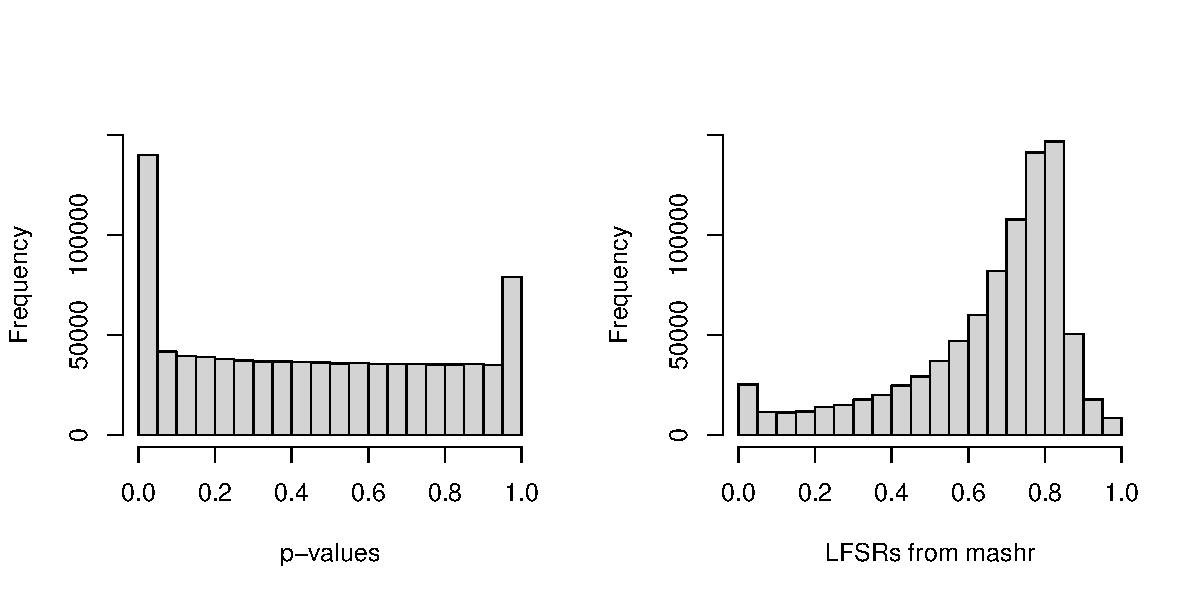
\includegraphics{Chapter_5_Analysis_files/figure-latex/pval-plot-1.pdf}
\caption{Comparison of distribution of p-values from LIMIX output
(left), and distribution of LFSRs from mashr output (right).}
\end{figure}

\normalsize

\hypertarget{multi-state-qtl-analysis}{%
\section{Multi-state QTL analysis}\label{multi-state-qtl-analysis}}

We use the \texttt{QTLExperiment()} constructor to create a
QTLExperiment from the estimates, standard errors, and LFSRs output from
\texttt{mashr}. The numeric assays `betas', `errors' and `lfsrs' are
specified as a list, and passed in through the \texttt{assays} argument.
\footnotesize

\begin{Shaded}
\begin{Highlighting}[]
\NormalTok{qtle }\OtherTok{\textless{}{-}} \FunctionTok{QTLExperiment}\NormalTok{(}
    \AttributeTok{assays=}\FunctionTok{list}\NormalTok{(}
        \AttributeTok{betas=}\NormalTok{betas.strong,}
        \AttributeTok{errors=}\NormalTok{errors.strong,}
        \AttributeTok{lfsrs=}\NormalTok{lfsrs.strong),}
    \AttributeTok{metadata=}\FunctionTok{list}\NormalTok{(}\AttributeTok{study=}\StringTok{"Natri\_Lung"}\NormalTok{))}
\NormalTok{qtle}
\end{Highlighting}
\end{Shaded}

\begin{verbatim}
## class: QTLExperiment 
## dim: 87888 10 
## metadata(1): study
## assays(3): betas errors lfsrs
## rownames(87888): ENSG00000178980|rs11671137 ENSG00000105486|rs17304898
##   ... ENSG00000144504|rs35561942 ENSG00000026508|rs111657272
## rowData names(2): variant_id feature_id
## colnames(10): endothelial_arteriole endothelial_venule ...
##   mesenchymal_AdventitialFB mesenchymal_AlveolarFB
## colData names(1): state_id
\end{verbatim}

\normalsize

As the basic operations of \textbf{\texttt{QTLExperiment}} and
\textbf{\texttt{multistateQTL}} have been discussed in Chapter 4, we
will briefly perform the necessary filtering and calculations.\\
We begin by updating the colData of the object to include lineage and
cell-types. \footnotesize

\begin{Shaded}
\begin{Highlighting}[]
\FunctionTok{head}\NormalTok{(}\FunctionTok{colnames}\NormalTok{(qtle))}
\end{Highlighting}
\end{Shaded}

\begin{verbatim}
## [1] "endothelial_arteriole"                
## [2] "endothelial_venule"                   
## [3] "epithelial_AT2"                       
## [4] "epithelial_Ciliated"                  
## [5] "epithelial_Secretory-SCGB1A1+SCGB3A2+"
## [6] "immune_Inflammatorymonocyte"
\end{verbatim}

\begin{Shaded}
\begin{Highlighting}[]
\CommentTok{\# Split state\_id into lineage and cell type (state)}
\NormalTok{qtle}\SpecialCharTok{$}\NormalTok{lineage }\OtherTok{\textless{}{-}} \FunctionTok{sapply}\NormalTok{(}\FunctionTok{strsplit}\NormalTok{(}\FunctionTok{state\_id}\NormalTok{(qtle), }\StringTok{"\_"}\NormalTok{), }\StringTok{"["}\NormalTok{, }\DecValTok{1}\NormalTok{)}
\FunctionTok{state\_id}\NormalTok{(qtle) }\OtherTok{\textless{}{-}} \FunctionTok{sapply}\NormalTok{(}\FunctionTok{strsplit}\NormalTok{(}\FunctionTok{state\_id}\NormalTok{(qtle), }\StringTok{"\_"}\NormalTok{), }\StringTok{"["}\NormalTok{, }\DecValTok{2}\NormalTok{)}
\FunctionTok{head}\NormalTok{(}\FunctionTok{colData}\NormalTok{(qtle))}
\end{Highlighting}
\end{Shaded}

\begin{verbatim}
## DataFrame with 6 rows and 2 columns
##                                          state_id     lineage
##                                       <character> <character>
## arteriole                               arteriole endothelial
## venule                                     venule endothelial
## AT2                                           AT2  epithelial
## Ciliated                                 Ciliated  epithelial
## Secretory-SCGB1A1+SCGB3A2+ Secretory-SCGB1A1+SC..  epithelial
## Inflammatorymonocyte         Inflammatorymonocyte      immune
\end{verbatim}

\normalsize

\hypertarget{plotting-global-sharing}{%
\subsection{Plotting global sharing}\label{plotting-global-sharing}}

A main aim of multi-state eQTL analysis is to better understand the
relationship between states. One way to measure this is by the
proportion of eQTL effects which are shared between pairs of states.

We begin by calling significance, using a threshold of 0.05 for the
LFSRs. We then filter to only rows with some significant states, and
calculate the pairwise sharing using \texttt{runPairwiseSharing()}. The
function \texttt{plotPairwiseSharing()} produces a heatmap showing the
proportion of significant eQTLs which are shared for each pairwise
combination of states. This can help us to understand the relationship
between the cell-types by their eQTL results. As the columns (and rows)
of the plot are clustered, we can see which states are most related. For
example, the states from the lineage `mesenchymal' have less sharing
than the immune cell-types.

\footnotesize

\begin{Shaded}
\begin{Highlighting}[]
\NormalTok{qtle }\OtherTok{\textless{}{-}} \FunctionTok{callSignificance}\NormalTok{(qtle, }\AttributeTok{assay=}\StringTok{"lfsrs"}\NormalTok{, }\AttributeTok{thresh=}\FloatTok{0.05}\NormalTok{)}

\NormalTok{qtle\_sig }\OtherTok{\textless{}{-}} \FunctionTok{getSignificant}\NormalTok{(qtle)}
\NormalTok{qtle\_top }\OtherTok{\textless{}{-}} \FunctionTok{runPairwiseSharing}\NormalTok{(qtle\_sig)}

\FunctionTok{dim}\NormalTok{(qtle\_top)}
\end{Highlighting}
\end{Shaded}

\begin{verbatim}
## [1] 4648   10
\end{verbatim}

\begin{Shaded}
\begin{Highlighting}[]
\FunctionTok{plotPairwiseSharing}\NormalTok{(qtle\_top, }\AttributeTok{annotateColsBy=}\FunctionTok{c}\NormalTok{(}\StringTok{"nSignificant"}\NormalTok{, }\StringTok{"lineage"}\NormalTok{))}
\end{Highlighting}
\end{Shaded}

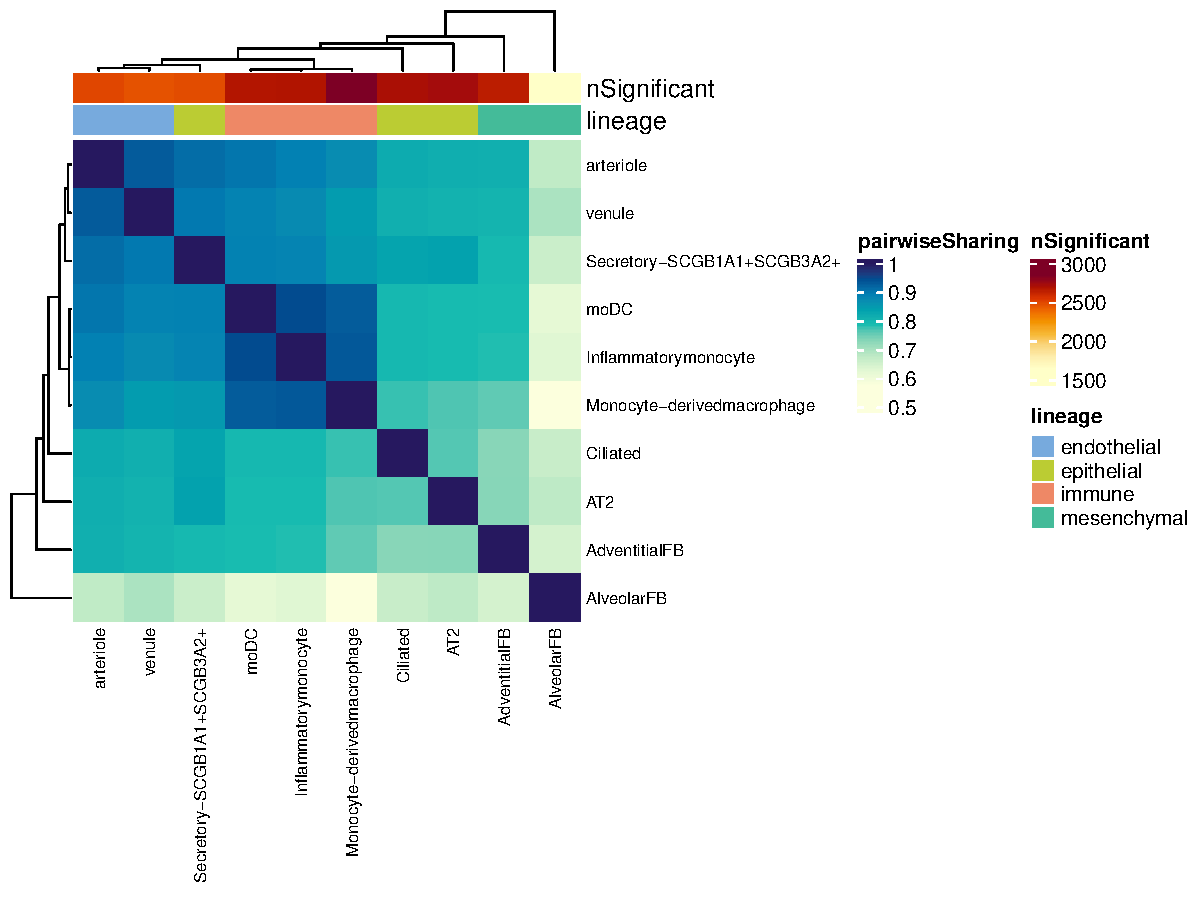
\includegraphics{Chapter_5_Analysis_files/figure-latex/plot-pairwise-lung-1.pdf}
\normalsize \footnotesize

\begin{Shaded}
\begin{Highlighting}[]
\FunctionTok{plotUpSet}\NormalTok{(qtle\_top, }\AttributeTok{annotateColsBy=}\FunctionTok{c}\NormalTok{(}\StringTok{"nSignificant"}\NormalTok{, }\StringTok{"lineage"}\NormalTok{))}
\end{Highlighting}
\end{Shaded}

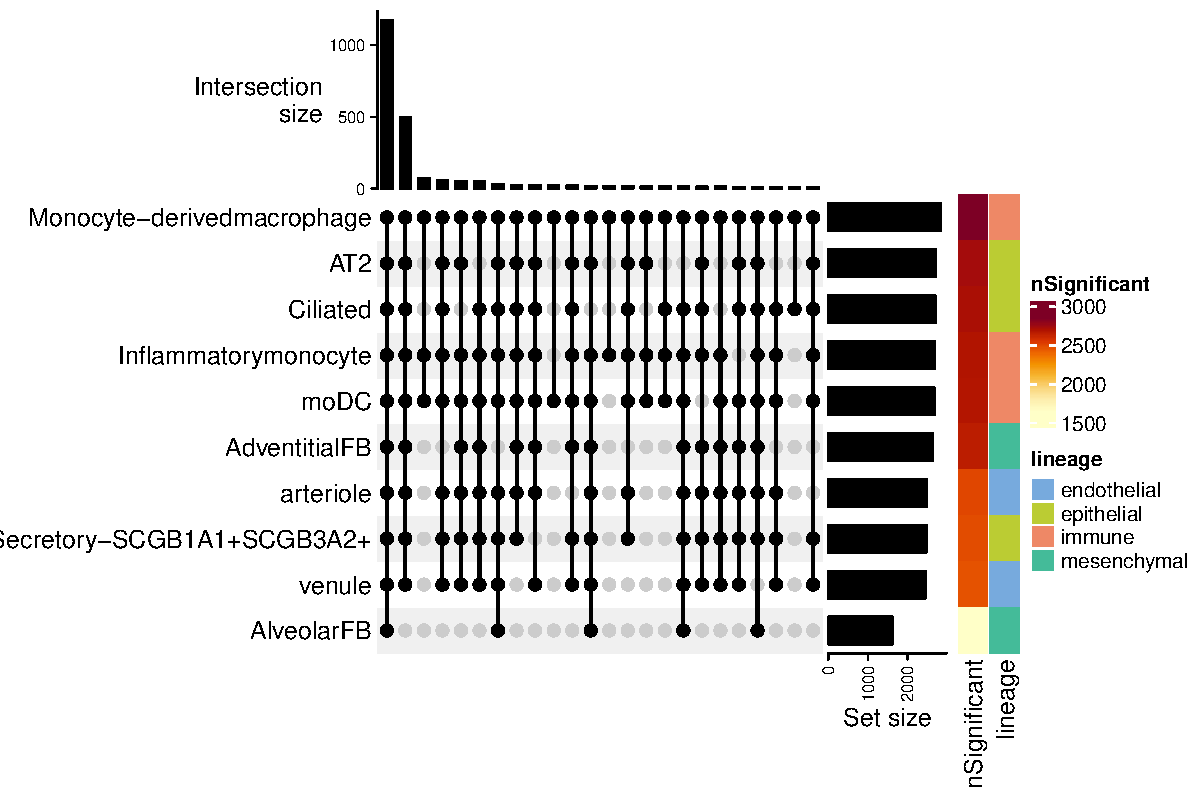
\includegraphics{Chapter_5_Analysis_files/figure-latex/plot-upset-lung-1.pdf}
\normalsize

\hypertarget{characterising-multi-state-qtl-patterns}{%
\subsection{Characterising multi-state QTL
patterns}\label{characterising-multi-state-qtl-patterns}}

After using \texttt{runTestMetrics()} to characterise eQTLs into
`unique', `multi-state' or `global', we can see that the majority of
eQTLs are unique. \footnotesize

\begin{Shaded}
\begin{Highlighting}[]
\NormalTok{qtle\_top }\OtherTok{\textless{}{-}} \FunctionTok{runTestMetrics}\NormalTok{(qtle\_top)}

\FunctionTok{table}\NormalTok{(}\FunctionTok{rowData}\NormalTok{(qtle\_top)}\SpecialCharTok{$}\NormalTok{qtl\_type)}
\end{Highlighting}
\end{Shaded}

\begin{verbatim}
## 
##        global_shared multistate_diverging    multistate_shared 
##                 1176                   99                 1713 
##               unique 
##                 1660
\end{verbatim}

\normalsize
\footnotesize

\normalsize

We can subset to just the unique eQTLs and plot a heatmap of these beta
values. This shows that some states have unique eQTLs which have strong
effects on the gene expression. For example, the state `AdventitialFB'
has a number of unique eQTLs which cause an increase in the expression
of a gene, as well as eQTLs that result in a decrease in gene
expression.

\footnotesize

\begin{Shaded}
\begin{Highlighting}[]
\NormalTok{qtle\_top\_unique }\OtherTok{\textless{}{-}} \FunctionTok{subset}\NormalTok{(qtle\_top, qtl\_type\_simple }\SpecialCharTok{==} \StringTok{"unique"}\NormalTok{)}

\FunctionTok{plotQTLClusters}\NormalTok{(}
\NormalTok{    qtle\_top\_unique, }
    \AttributeTok{annotateColsBy=}\StringTok{"lineage"}\NormalTok{,}
    \AttributeTok{annotateRowsBy=}\FunctionTok{c}\NormalTok{(}\StringTok{"qtl\_type"}\NormalTok{))}
\end{Highlighting}
\end{Shaded}

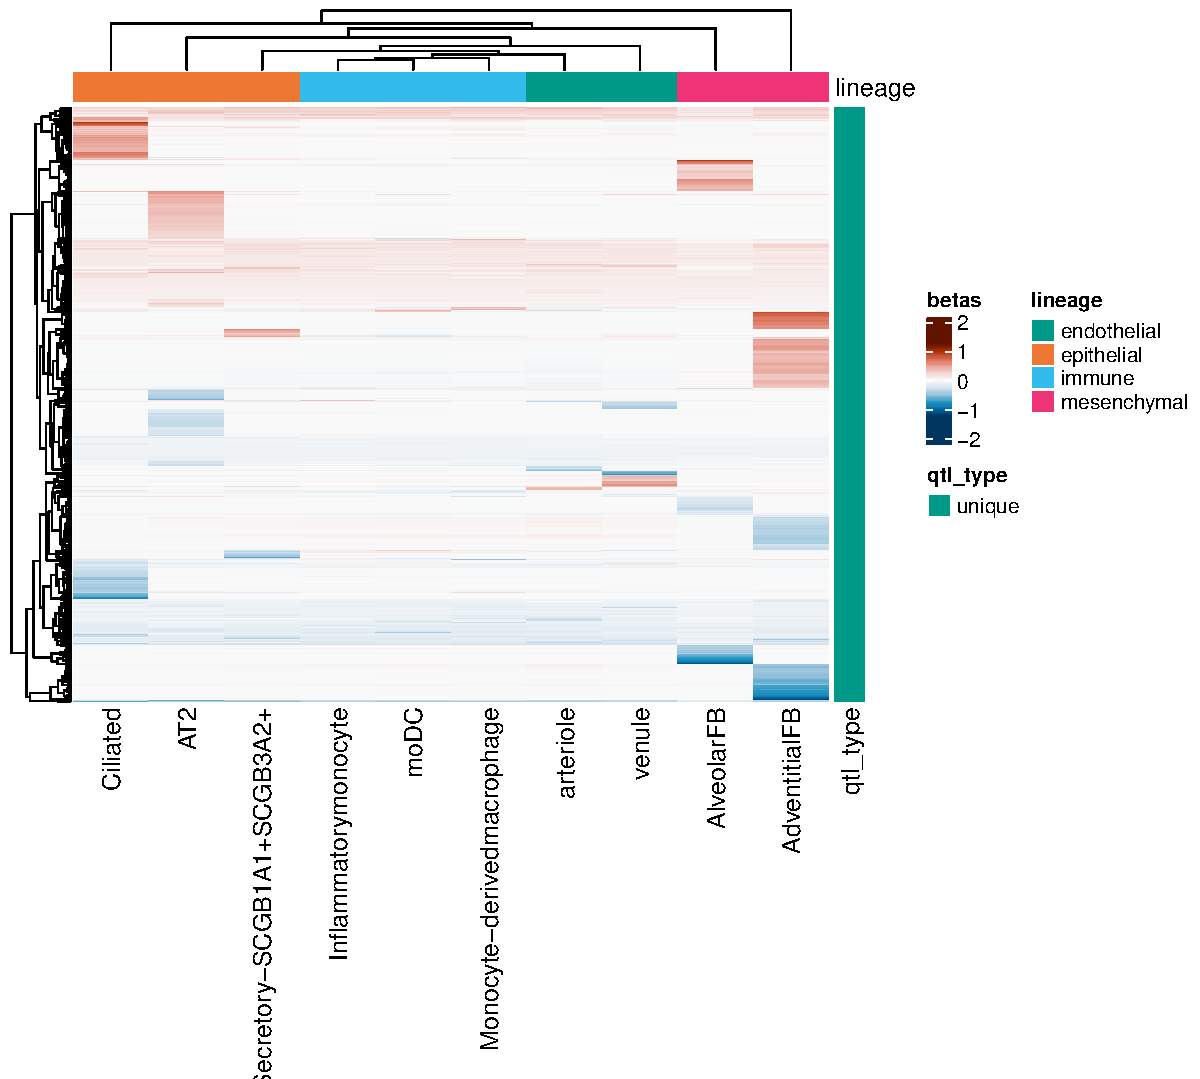
\includegraphics{Chapter_5_Analysis_files/figure-latex/plot-unique-lung-1.pdf}
\normalsize

\hypertarget{conclusion}{%
\section{Conclusion}\label{conclusion}}

This concludes our demonstration of \textbf{\texttt{QTLExperiment}} and
\textbf{\texttt{multistateQTL}}. In this chapter, we analysed a data set
where states represent different cell-types, outlining the additional
challenge that comes with analysing single-cell data. We mentioned the
processing steps which are required before the multi-state QTL analysis
can begin, including quality control, batch correction, feature
selection, clustering, and principal component analysis. Notably, it is
necessary to annotate the cell-types in the data set so that these can
be used as the `states' in the multi-state eQTL analysis which follows.

We also provided a tutorial to run multivariate adaptive shrinkage using
functions from the \textbf{\texttt{multistateQTL}} package. This adjusts
the summary statistics from condition-by-condition results so that
patterns of sharing is learnt between states. Finally, we visualised the
multi-state eQTL data to identify patterns within the states, and gained
a deeper understanding of the impact genetic variants have across a
range of cell-types.

\end{document}
